\chapter{Dise'no e implementaci'on del servicio web}
\label{capitulocinco}
El desarrollo del servicio en el presente proyecto es para crear un nuevo servicio que garantiza la abstracci'on y la reutilizaci'on de la p'agina del SAGAA.

%El desarrollo del servicio web proporciona el analisis de las actividades y la comunicaci'on de la p'agina del SAGAA, a tr'aves de los dise'nos para ofrecer una explicaci'on logicamente coherencia e independiente.


\section{Identificar el candidato a servicio}
Para identificar el candidato a servicio sin embargo la experiencia y la habilidad en el desarrollo de servicios web.\\
El presente proyecto tiene el objetivo de optimizar los procesos de llenar la planilla de notas en la p'agina del SAGAA como se ha mencionado anteriormente en el capitulo \ref{capitulotres}.
%Para el presente proyecto, analizar cada proceso de la p'agina del SAGAA, es identificar la ubicaci'on y descripci'on del detalle de la interfaz. Para el documento de interfaz se utilizan las operaciones que soportan el servicio web y el documento de enlace, se muestra una interfaz abstracta con un conjunto de protocolos.
Para verificar si el servicio es 'util se realiza el cuestionario, el c'ual se desarrolla en el anexo \ref{cuestionario}.
Despues de lo mencionado anteriormente se realiza la lista de requerimientos para el servicio web estos se mencionan a continuaci'on.

\subsection{Requerimientos del servicio web}
\label{requerimientoServicio}
Los requerimientos que se muestran a continuaci'on son un conjunto de servicios los cuales se obtienen a partir de los procesos de llenar la planilla de notas como se ha explicado anteriormente en el capitulo \ref{capitulotres}. 
\begin{enumerate}
%\item Realizar la sesi'on del usuario.
%\item Obtener los datos de la gesti'on de la planilla de nota.
%\item Seleccionar la gesti'on de la planilla de nota.
\item Descargar la planilla de notas seg'un la gesti'on y la carrera corespondiente.
\item Obtener datos de la p'agina del SAGAA para la unidad de datos para compartir la informaci'on de la planilla de notas.
\item Adjuntar la planilla de nota modificada en la p'agina del SAGAA.
\end{enumerate}
Una vez concluido con los requerimientos se avanza a la etapa de dise'no del servicio web.

\section{Dise'no del servicio}
El dise'no del servicio describe la informaci'on al env'iar los mensajes de entrada y salida  de la p'agina del SAGAA al realizar el proceso de llenar la planilla de notas. Las etapas del dise'no de servicio son la: interfaz l'ogica, mensajes, el desarrollo de WSDL y la especificaci'on del servicio. A continuaci'on se explican cada etapa.


\subsection{La etapa de dise'no de interfaz l'ogica}
El dise'no de interfaz l'ogica es la comunicaci'on entre el cliente y el servidor. El servidor almacena informaci'on de la p'agina del SAGAA. Para explicar los procesos para llenar la planilla de notas.

\begin{itemize}
\item \textit{El Dise'no de interfaz l'ogica del proceso de descargar la planilla de notas} se representa en la siguiente figura \ref{fig:DisenoDescargar2} el cual es la secuencia de peticiones ordenadas, los par'ametros de entrada y salida o mensajes y  las direcciones de url.
% Para realizar las peticiones de descarga de la planilla de notas y obtener los datos para realizar el siguiente proceso.
\begin{figure}[H]
\centering
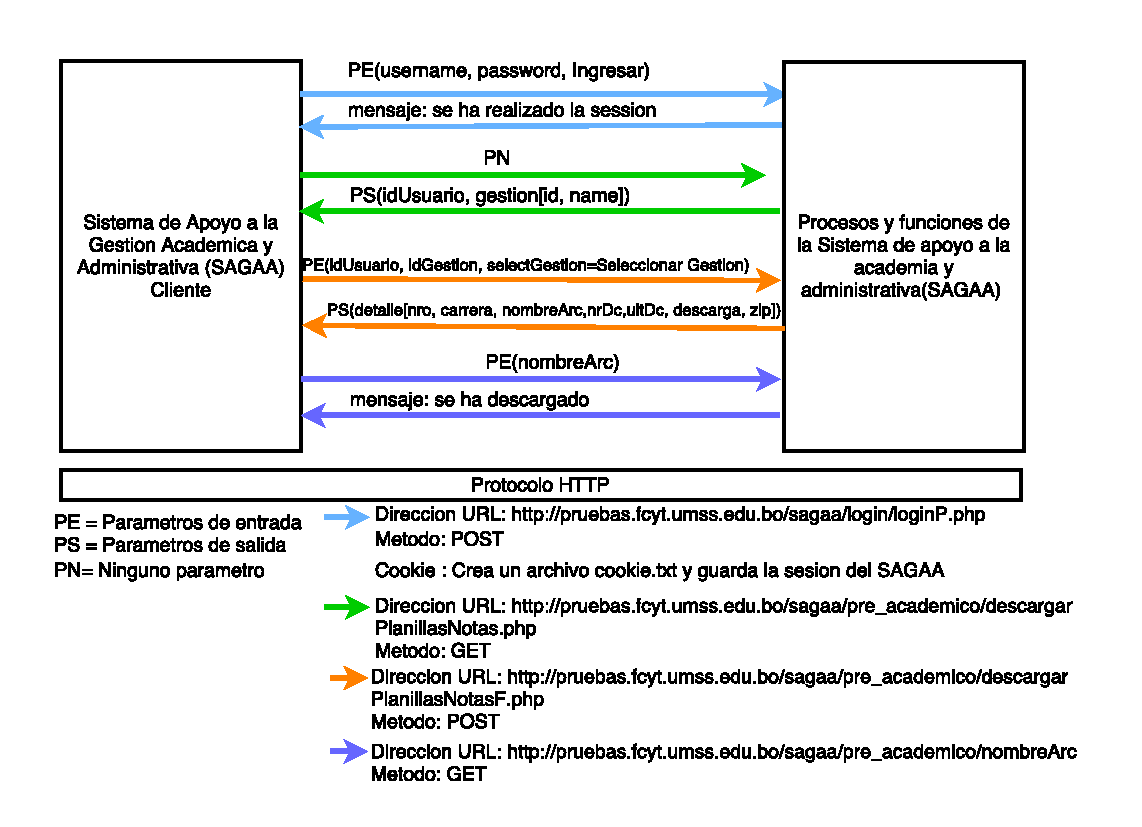
\includegraphics[width=0.7\textwidth]{disenoOperacionDescarga.pdf}
\captionsetup{justification=centering, margin=2cm}
\caption{Dise'no de interfaz l'ogico para descargar la planilla de nota, Fuente: Elaboraci'on propia}
\label{fig:DisenoDescargar2}
\end{figure}

\item \textbf{Dise'no de interfaz l'ogica de adjuntar la planilla de notas,} describe la secuencia de peticiones ordenadas y los parametros de entrada y salida o mensajes y las direcciones de url. Como se muestra en la figura \ref{fig:DisenoSubir}.
% a continuaci'on se expone la secuencia de peticiones ordenas y los parametros de entrada y salida o mensajes y las direcciones de url para realizar el proceso de subir la planilla de notas a la p'agina del SAGAA.
\begin{figure}[H]
\centering
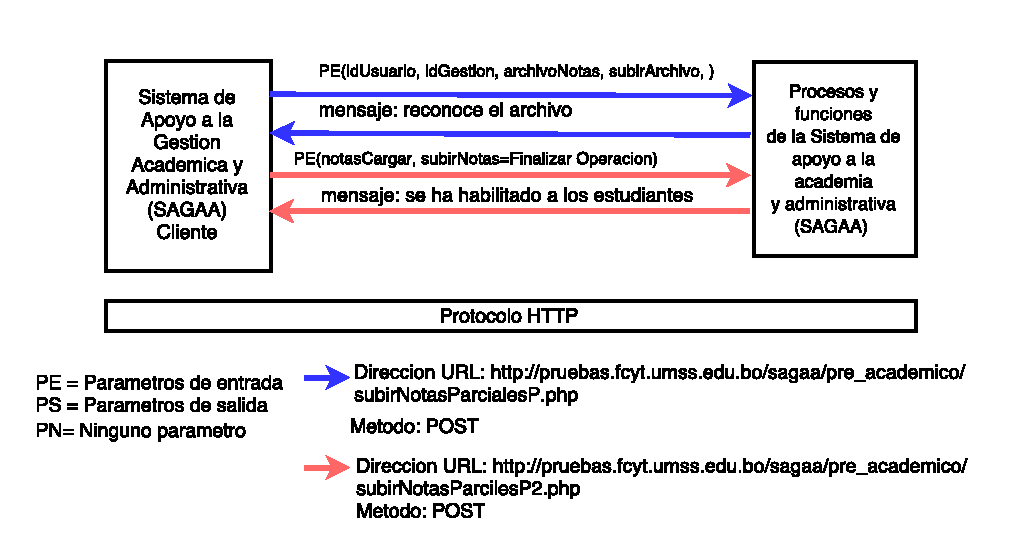
\includegraphics[width=0.6\textwidth]{disenoOperacionSubir.pdf}
\captionsetup{justification=centering, margin=2cm}
\caption{Dise'no de interfaz l'ogico para adjuntar la planilla de notas, Fuente: Elaboraci'on propia}
\label{fig:DisenoSubir}
\end{figure}
\end{itemize}

\subsection{Dise'no de mensaje}
El dise'no de mensaje define la estructura de los mensajes que transcurren en la  comunicaci'on del cliente y servidor cuando se realiza una petici'on.Los mensajes ayudan a mostrar los estados  de la petici'on si es correcta, incorrecta y excepciones. En la siguiente figura \ref{fig:DisenoMensaje} se muestra los mensajes del proceso de llenar la planilla de notas.

\begin{figure}[H]
\centering
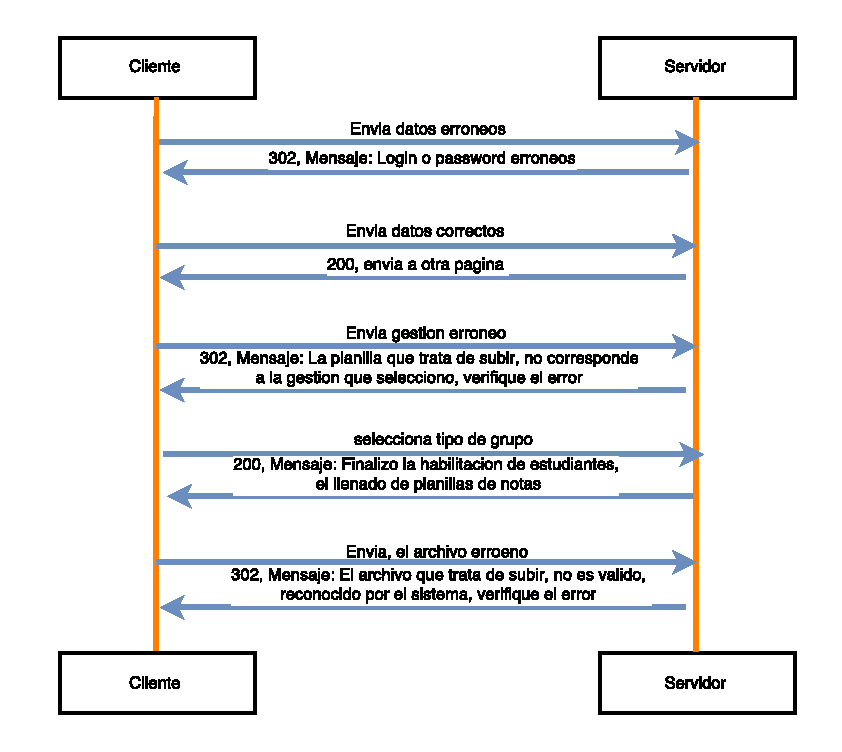
\includegraphics[width=0.6\textwidth]{disenoMensaje.pdf}
\captionsetup{justification=centering, margin=2cm}
\caption{Dise'no de mensaje de entradas, salidas y excepciones, Fuente: Elaboraci'on propia}
\label{fig:DisenoMensaje}
\end{figure}

\subsection{Desarrollo de WSDL}
El desarrollo de WSDL no ha utilizadola estestructura de desarrollo XML  porque utiliza el protocolo REST para la implementaci'on del servicio. El desarrollo de WSDL describe de la interfaz abstracta para llenar la planilla de notas como se explican a continuaci'on en el documento de interface y el documento de enlace.
\begin{itemize}
\item \textbf{Documento de interface}\\
El documento de interface define las operaciones del proceso de llenar la planilla de notas lo cual se dividen en tres procesos los cuales son:
\begin{enumerate}[\bfseries Pr{o}ceso 1:]
 \item Secuencia de procesos para  descargar la planilla de notas en el formato .sis de la p'agina del SAGAA. En la figura \ref{fig:Proceso1}.
 
 \begin{figure}[H]
 \centering
 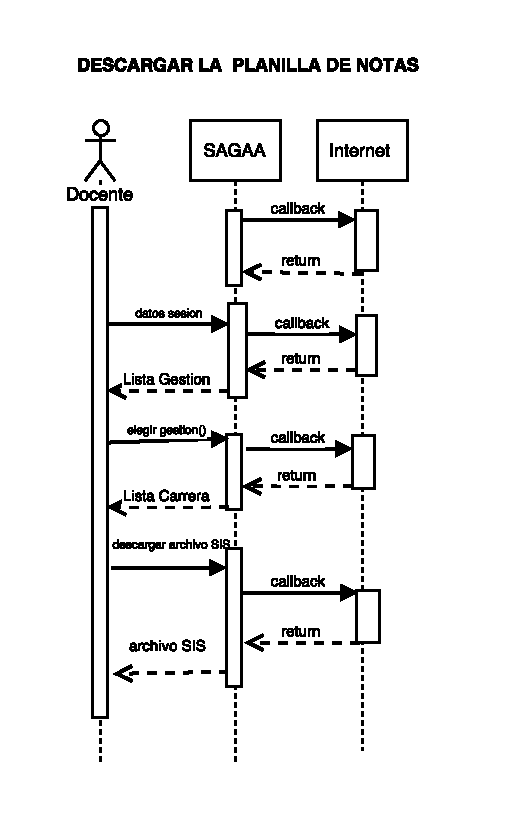
\includegraphics[width=0.3\textwidth]{SdescargarLlenadoNota.pdf}
 \captionsetup{justification=centering,margin=2cm}
 \caption{Proceso de descargar Planilla Notas. Figura: Elaboraci'on propia}
 \label{fig:Proceso1}
 \end{figure}
 
 \item En este proceso se muestran los pasos para modificar la planilla de notas y se ha utilizado la aplicaci'on del Transcriptor.exe para modificar la planilla de notas como se observa en la siguiente figura \ref{fig:Proceso2}.
 
 \begin{figure}[H]
 \centering
 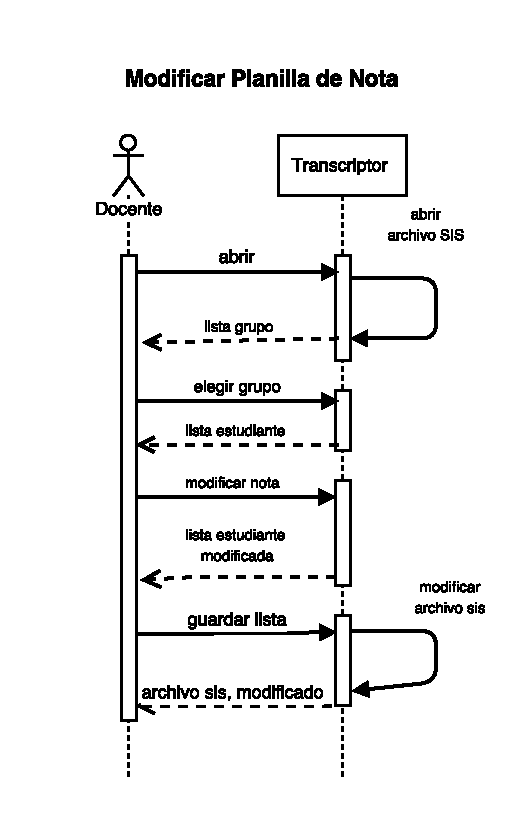
\includegraphics[width=0.3\textwidth]{DSmodificarPlanila.pdf}
 \captionsetup{justification=centering,margin=2cm}
 \caption{Proceso de modificar la Planilla de Notas, Fuente: Elaboraci'on propia}
 \label{fig:Proceso2}
 \end{figure}
   
  \item La ultima secuencia de pasos para adjuntar el archivo de planilla de notas en la p'agina del SAGAA se muestra en la figura \ref{fig:Proceso3}.
  
\begin{figure}[H]
\centering
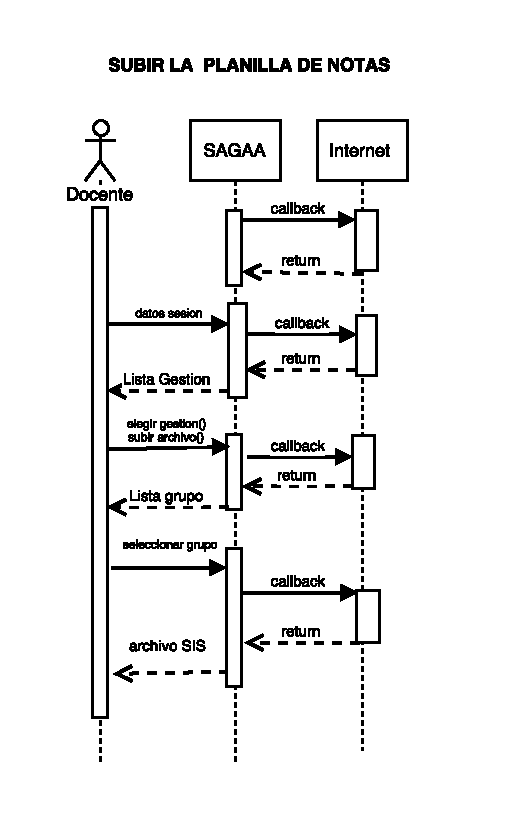
\includegraphics[width=0.3\textwidth]{DSsubirPlanilla.pdf}
\captionsetup{justification=centering, margin=2cm}
\caption{Proceso de subir a la p'agina del SAGAA, Fuente: Elaboraci'on propia}
 \label{fig:Proceso3}
 \end{figure}
\end{enumerate}

\item \textbf{Documento enlace}\\
El documento de enlace es la interfaz abstracta de un conjunto concreto de protocolos los cuales especifican los detalles t'ecnicos de la comunicaci'on entre la p'agina del SAGAA y el servidor. El servidor es donde se almacena la informaci'on solicitada. La interfaz abstracta se representa en la siguiente figura \ref{fig:Comunicacion}.
\begin{figure}[H]
\centering
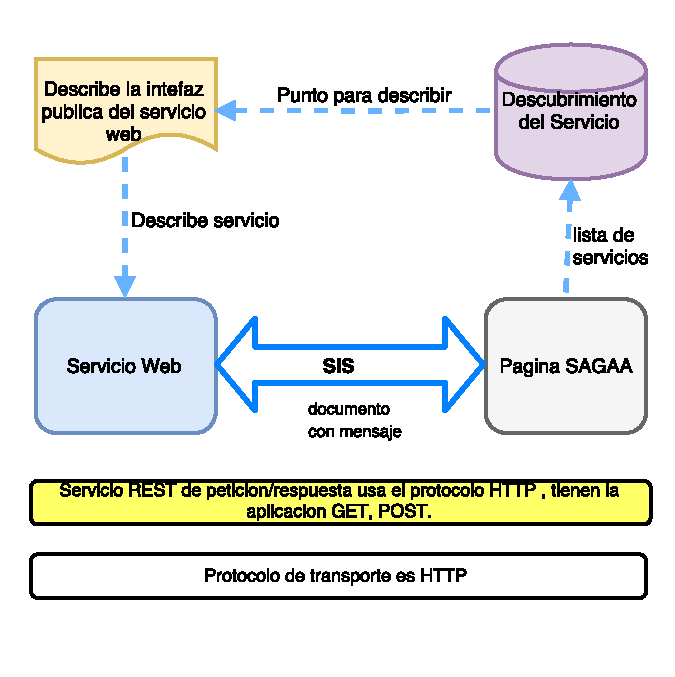
\includegraphics[width=0.4\textwidth]{comunicacioProtocolo.pdf}
\captionsetup{justification=centering, margin=2cm}
\caption{Protocolos de servicio, Fuente: Elaboraci'on propia}
\label{fig:Comunicacion}
\end{figure}

%En la figura \ref{fig:Comunicacion}, se muestran los protocolos que utilizan la p'agina del SAGAA para realizar el proceso de llenar la planilla de notas.

\end{itemize}

\subsection{Especificaci'on del servicio}
En la etapa de especificaci'on del servicio describe las construcci'on de servicios las cuales son: formular el bosquejo de trabajo, lista de servicio y especificaci'on de servicio.
\begin{itemize}
\item \textbf{Formular el bosquejo de flujo de trabajo}\\
A partir de los requerimientos se ha desarrollado un servicio compuesto el c'ual es la base para el nuevo diagrama de flujo de trabajo. Este servicio compuesto describe la secuencia de pasos de llenar la planilla de notas como se observa en la siguiente figura \ref{fig:flujoTrabajo1}.

\begin{figure}[H]
\centering
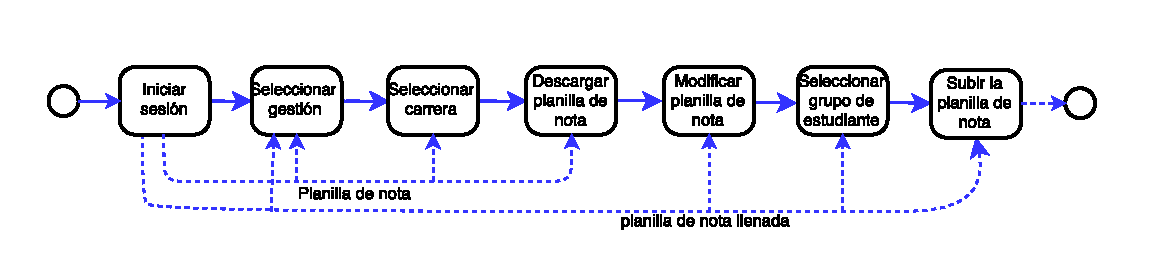
\includegraphics[width=0.9\textwidth]{flujoTrabajo1.pdf}
\captionsetup{justification=centering, margin=2cm}
\caption{Diagrama de flujo de trabajo, Fuente: Elaboraci'on propia}
\label{fig:flujoTrabajo1}
\end{figure}

\item \textbf{Descubrir el servicio}\\
\label{Lista}
Durante la etapa de descubrir el servicio se ha buscado el catalogo o registros para realizar el proceso de llenar la planilla de notas en la p'agina del SAGAA el c'ual se ha obtenido a partir del capitulo \ref{capitulotres}. A continuaci'on la siguiente lista de servicio son:\\

\textbf{Lista de servicio}
\begin{enumerate}
\item Realizar la sesi'on.
\item Listar la gesti'on.
\item Seleccionar la gesti'on
\item Listar las carreras.
\item Seleccionar carrera, para descargar la planilla de notas.
%\item Crear una unidad de datos de la planilla de notas.
\item Subir la planilla de nota modificado.
\end{enumerate}

\item \textbf{Seleccionar el servicio}\\
\label{Especificaciones}
A partir de la lista de servicios se han seleccionado los  candidatos a servicios. Los cuales son los siguientes indices.\\

\begin{enumerate}
\item Para descargar la planilla de notas se realizan la sesi'on del docente,  seleccionar la gesti'on, seleccionar la carrera y por ultimo se descarga la planilla de nota.
\item Modificar la planilla de notas se ralizo a trav'es de la aplicaci'on m'ovil reconocer la planilla de notas, mostrar, modificar y enviar la planilla de notas modificada a la p'agina del SAGAA.
%Modificar la planilla de notas es donde se guarda la planilla de datos localmente, reconoce la planilla de notas, y con la ayuda de la aplicaci'on m'ovil mostrar y modificar la planilla de notas y enviar la planilla de notas modificada a la p'agina del SAGAA.
\item Para subir la planilla de notas primeramente se elige el grupo de materia, luego se adjunta la planilla y por ultimo se selecciona el tipo de grupo para publicar la planilla de notas en la p'agina del SAGAA.
\end{enumerate}
\end{itemize}
%hasta aqui	
\subsection{Implementaci'on y despliegue del servicio}
Al concluir con los dise'nos de interface abstracta se  realizan las etapas de refinar el flujo de trabajo y crear el programa de flujo de trabajo.
\begin{itemize}

\item \textbf{Refinar el flujo de trabajo}\\
A partir de  seleccionar el servicio se realiza el dise'no del servicio. Cada diagrama mejora el detalle y la descripci'on abstracta de cada servicio seleccionado. Cada diagramas mejoran el detalle y la discripci'on abstracta de cada especificaci'on del servicio seleccionado. A continuaci'on se explican cada diagrama de flujo de trabajo.
\begin{itemize}
\item \textit{Descarga la planilla de notas} es la secuencia de procesos para descargar la planilla de notas el c'ual se representa a trav'es del diagrama de flujos de trabajo como se muestra en la siguiente figura \ref{fig:FlujoTrabajoDescargar}.
\begin{figure}[H]
\centering
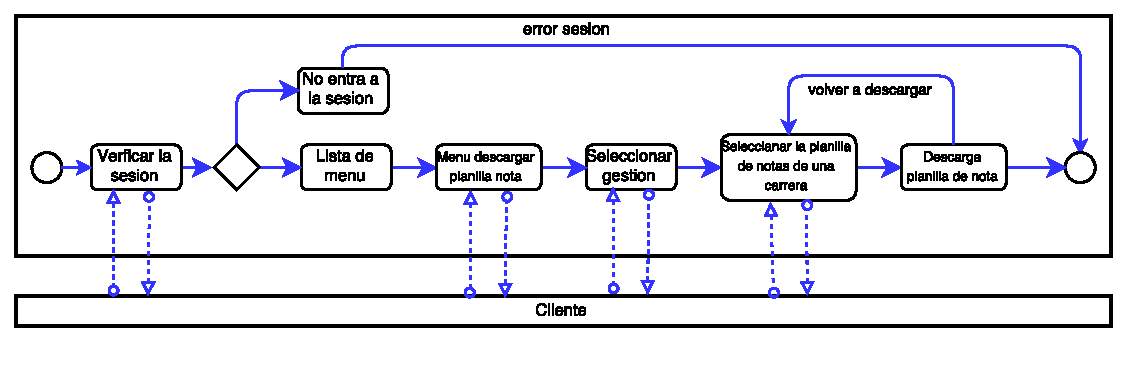
\includegraphics[width=0.8\textwidth]{flujoTrabajoDescarga.pdf}
\captionsetup{justification=centering, margin=2cm}
\caption{Dise'no de flujo de trabajo de descarga de la planilla de notas, Fuente: Elaboraci'on propia}
\label{fig:FlujoTrabajoDescargar}
\end{figure}

\item \textit{Dise'no de modificar la planilla de notas} utiliza la aplicaci'on del Transcriptor.exe el c'ual tiene una secuencia de procesos. En la siguiente figura \ref{fig:FlujoTrabajoModificar} el diagrama de flujo de trabajo. .
\begin{figure}[H]
\centering
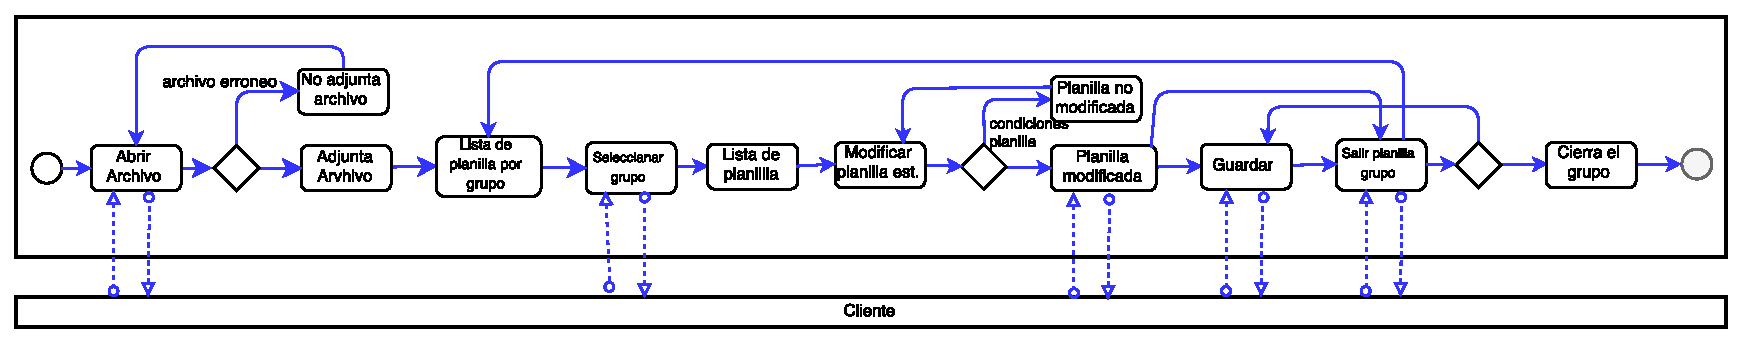
\includegraphics[width=0.8\textwidth]{flujoTrabajoModificar.pdf}
\captionsetup{justification=centering, margin=2cm}
\caption{Dise'no de flujo de trabajo de la descarga de la planilla de notas, Fuente: Elaboraci'on propia}
\label{fig:FlujoTrabajoModificar}
\end{figure}

\item \textit{Dise'no para adjuntar la planilla de notas} son pasos secuenciales para publicar la planilla de notas el c'ual se representa a trav'es de la figura \ref{fig:FlujoTrabajoSubir2}.
\begin{figure}[H]
\centering
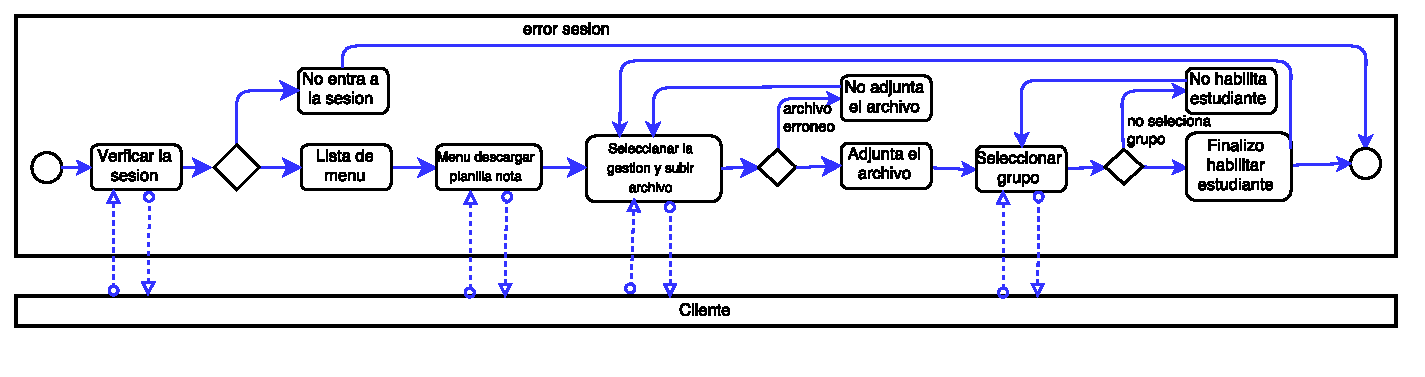
\includegraphics[width=0.8\textwidth]{flujoTrabajoSubir.pdf}
\captionsetup{justification=centering, margin=2cm}
\caption{Dise'no de flujo de trabajo de subir la planilla de notas, Fuente: Elaboraci'on propia}
\label{fig:FlujoTrabajoSubir2}
\end{figure}
\end{itemize}

\item \textbf{Crear un programa de flujo de trabajo}
\label{CrearFlujo}
el diagrama para crear un programa de flujo de trabajo es la uni'on de los servicios seleccionados anteriormente el dise'no de flujo de trabajo de descargar, modificar y adjuntar. Se representa en la siguientes figuras\ref{fig:FlujoTrabajoPlanilla} el crear un programa de flujo de trabajo. 
\begin{figure}[H]
\centering
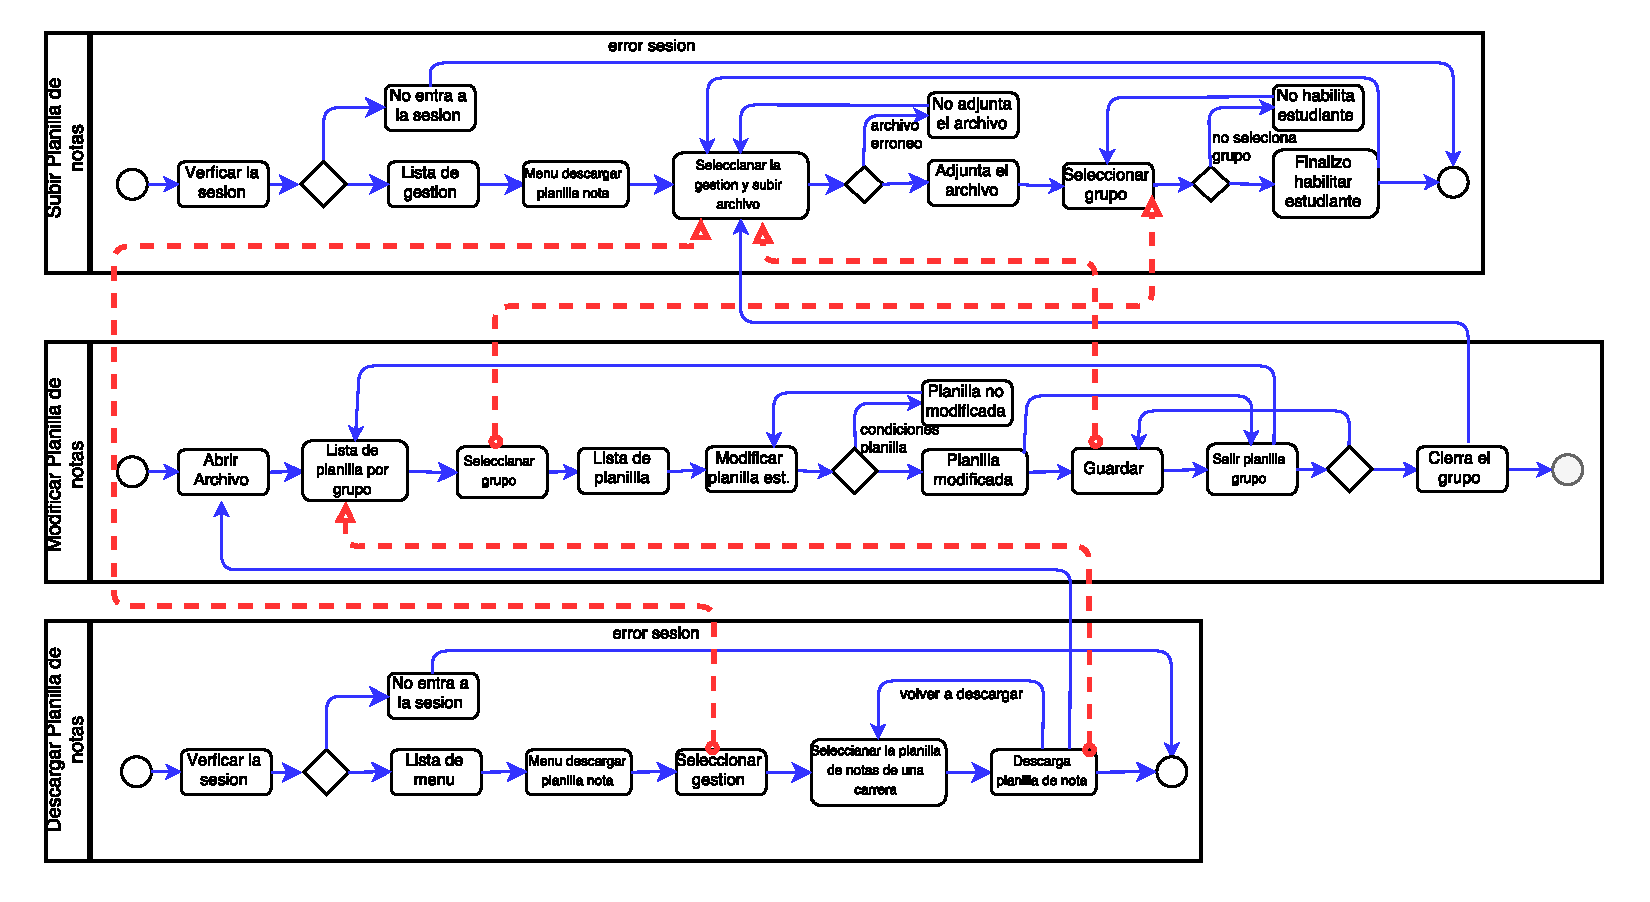
\includegraphics[width=1\textwidth]{flujoTrabajoPlanilla.pdf}
\captionsetup{justification=centering, margin=2cm}
\caption{Dise'no de flujo de trabajo planilla de notas, Fuente: Elaboraci'on propia}
\label{fig:FlujoTrabajoPlanilla}
\end{figure}
\end{itemize}
En la figura \ref{fig:FlujoTrabajoPlanilla} se representa los tres procesos, las flechas de punteada, es la comunicaci'on entre procesos y par'ametros que comparten entre ellos, para el desarrollo del servicio web.
%Hay que aumentar los datos del json.
%\subsection{El dise'no de unidad de datos de servicio} 
%El formato que se utiliza para intercambiar informaci'on, es un formato ligero conocido como \textbf{JSON} es representado en objetos y arreglos.// 

%La unidad de datos de la p'agina del SAGAA es definida con etiquetas y tiene la extensi'on sis, para el presente proyecto se ha utilizado para la estructura predefinida.//

%La unidad de datos sis, ha sido modificado para convertirlo en el formato json, y asi la aplicaci'on m'ovil pueda reconocerlo.

\section{Desarrollo de la implementaci'on del servicio}
Para el desarrollo de la implementaci'on del servicio se realiza a partir de la figura \ref{fig:FlujoTrabajoPlanilla}, el c'ual describe la selecci'on del servicio. La figura \ref{fig:FlujoTrabajoImplementar} representa el diagrama de flujo para la implementaci'on del servicio.


\begin{figure}[H]
\centering
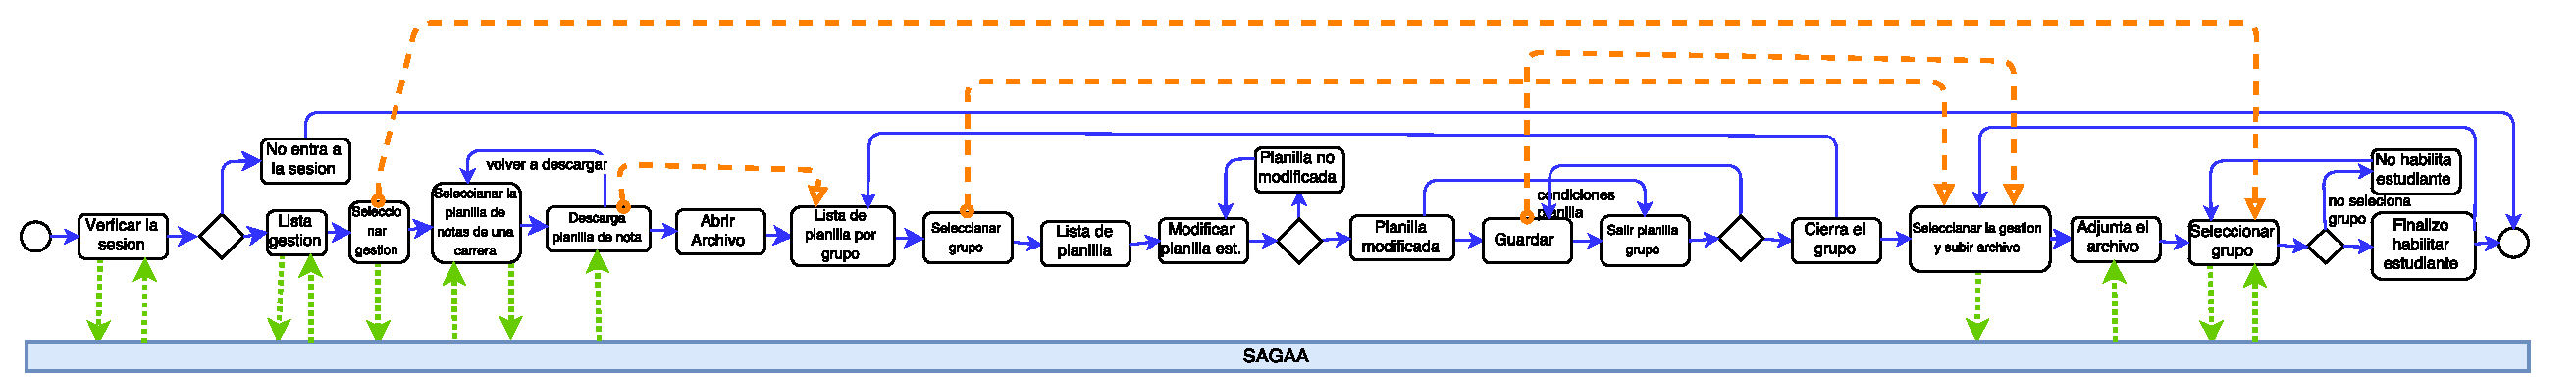
\includegraphics[width=1\textwidth]{flujoTrabajoImplementar.pdf}
\captionsetup{justification=centering, margin=2cm}
\caption{Dise'no de flujo de trabajo planilla de notas para la implementaci'on, Fuente: Elaboraci'on propia}
\label{fig:FlujoTrabajoImplementar}
\end{figure}

La figura \ref{fig:FlujoTrabajoImplementar} es la secuencia de proceso para el desarrollo del servicio web. Las lineas naranjas son par'ametros que comparten entre actividades.

\subsection{Herramientas y configuraci'on para la implementaci'ion del servicio}
Para el presente proyecto se ha utilizado el lenguaje de programaci'on de javascript y express es un framework de Nodejs. El express es una extensi'on de conecci'on con muchos m'etodos de la arquitectura de REST y intercambio de informaci'on a su disposici'on.

\begin{itemize}
\item \textbf{Arquitectura del framework Express} express utiliza la arquitectura de modelo, vista y controlador definida como MVC. 

\begin{figure}[H]
\centering
 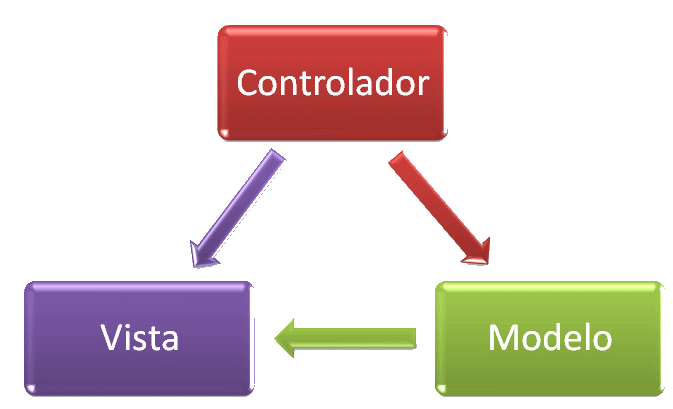
\includegraphics[width=0.4\textwidth]{arqExpress.png}
 \captionsetup{justification=centering,margin=2cm}
 \caption{Arquitectura de Express, adoptado para la realizaci'on del proyecto. Arquitectura de Express de \cite{Lopez2017}}
\end{figure}

Para el presente proyecto se ha implementado la parte del modelo para explicar la comunicaci'on del servicio web como se muestra  en la arquitectura de Nodejs en la figura \ref{fig:arqNodejs}..

\item\textbf{Arquitectura de Nodejs} utiliza la arquitectura orientado cliente/servidor.

\begin{figure}[H]
\centering
 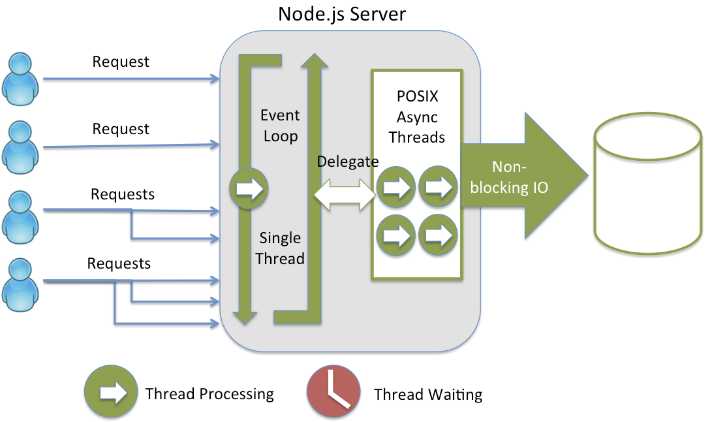
\includegraphics[width=0.6\textwidth]{arqNode.png}
 \captionsetup{justification=centering,margin=2cm}
 \caption{Arquitectura de NodeJs, adoptado para la realizaci'on del proyecto. Arquitectura de NodeJs de \cite{Munoz2013}}
 \label{fig:arqNodejs}
\end{figure}
En la arquitectura de Nodejs, analiza las peticiones de entrada y salida.
\end{itemize}

\subsection{Estructura del servicio web}
La estructura de servicio web utiliza la estructura de Ionic  tal como se ha mencionado anteriormente en el presente proyecto y  aumenta el archivo  server.js.
\begin{verbatim}
proyecto
    |--package.json (paquetes de plugin de NodeJS)
    |--plugins/ (Se guardan los plugins para el server)
    |--www/ (Código fuente principal)
    	|--archivo/ (guarda los archivos)
        |--js/ ( El código, Javascript de la aplicación)
            |--server.js
 \end{verbatim}

\subsection{Configuraci'on del servicio web}
Previamente se debe instalar node y npm para comenzar a realizar los siguientes comandos para configurar el servidor:

\begin{verbatim}
$ npm install -g express (instalar globalmente express)
$ touch server.js (crear el archivo server.js)
$ node server.js (ejecuta el server.js)
$ npm install nombre_plugins -g (instalar plugins necesarios para el proyecto)
\end{verbatim}
\subsection{Aplicar el servicio web en express}
Para la implementaci'on el servicio web se ha utilizado la herramienta de Curl, Cherrie y la cuenta de docente el cual ha sido proporcionada por la UPSI de la FCYT. Se ha utilizado el dise'no de flujo de trabajo de implementaci'on de planilla de notas de la figura  \ref{fig:FlujoTrabajoImplementar} el c'ual tiene los siguientes servicio web: 
\begin{itemize}
\item Verificar la sesi'on.
\item Listar la gesti'on. 
\item Seleccionar la gesti'on y devuelve la lista de las carreras.
\item Seleccionar la carrera de la planilla de notas para descargar planilla de notas. 
\item Filtrar y convertir la planilla de notas a unidades de datos de servicio json.
\item La planilla de notas con la unidad de datos modificados.
\item Crear una firma de clave para el servicio web.
\item Seleccionar la gesti'on y adjuntar planilla de notas modificada. 
\item Crear unidad de datos json.
\item Modificar los datos de la planilla de notas.
\item Configura el sesion de token.
\item Depende del anterior item seleccionar grupo para habilitar estudiante.
\end{itemize}
Cada servicio web es muy importante para lograr el objetivo general y se utilizan los datos del dise'no de interfaz l'ogico de la figura  \ref{fig:DisenoDescargar2} y el dise'no de interfaz l'ogica para adjuntar la planilla de notas de la figura \ref{fig:DisenoSubir} para realizar cada servicio web. Para mostar la implementaci'on del servicio web se explican las partes importantes a continuaci'on:
\begin{itemize}
\item \textit{Verificar la sesi'on} para verificar la sesion tenemos los siguientes datos: la direcci'on de url, el m'etodo que utiliza, los par'ametros y  agentes de autorizaci'on. Finalmente 'envia los datos mencionados a otra p'agina. 
\begin{verbatim}
var curl = new Curl(),
url  = 'http://pruebas.fcyt.umss.edu.bo/sagaa/login/loginP.php',
data = {
  'loginUsuario' : req.body.username,
  'claveUsuario' : req.body.password,
  'botonFormulario' : 'Ingresar'
};
curl.setOpt( Curl.option.URL, url );//direccion
curl.setOpt( Curl.option.FOLLOWLOCATION, true);//permite enviar a otra pagina
curl.setOpt( Curl.option.POST, 1);//metodo que utiliza
curl.setOpt( Curl.option.POSTFIELDS, data );//parametros 
curl.setOpt( Curl.option.HTTPHEADER, ['User-Agent: Mozilla/5.0',
'Content-Type: application/x-www-form-urlencoded'] );
// agentes de autorizacion
curl.setOpt( Curl.option.COOKIEFILE, 'pcb5r5tg8l1lbcjbqffr6hfm56'); 
// codigo de cookie de otra sesion, para obtener la sesion
curl.setOpt( Curl.option.COOKIEJAR, 'cookie.txt');
//guarda la cookie en el archivo txt
curl.on('end', function( statusCode, body, headers ) {
......
//respuesta de la comunicac'ion con el servidor del SAGAA
});
......
\end{verbatim}  
\item \textit{Seleccionar la gesti'on y adjuntar planilla de notas} para este servicio se conoce: la direcci'on de url, el m'etodo que utiliza, par'ametros encriptados, el httpheader para los agentes de autorizaci'on y la ubicaci'on de la planilla de notas para adjuntar.

\begin{verbatim}
....
dirA = '/home/geovanna/appSAGAA/appSAGAA/www/archivo/',
//ubicacion de la planilla de notas modificada
nameD = nombreAr,
idUsuario = usuarioId;
idGestion = gestionId;
url  = 'http://pruebas.fcyt.umss.edu.bo/sagaa/pre_academico/
subirNotasParcialesP.php';
curlS.setOpt( Curl.option.URL, url ); //direccion
curlS.setOpt( Curl.option.POST, 1); //metodo
curlS.setOpt( Curl.option.HTTPHEADER,['Connection: keep-alive',
'User-Agent: Mozilla/5.0','Content-Type: multipart/form-data;', 
'Cache-Control: max-age=0', 'Accept-Encoding: gzip, deflate']);
\\agentes de autorizacion
curlS.setOpt( Curl.option.HTTPPOST, [{name: 'idUsuario',
contents: idUsuario }, {name: 'idGestion', contents: idGestion },
{ name: 'archivoNotas', file: dirA + nameD, 
type: 'application/vnd.symbian.install'}, 
{ name: 'subirArchivo', contents: 'Subir Archivo'}]);
//estructura de parametros encriptados
curlS.setOpt( Curl.option.COOKIEFILE, 'cookie.txt');
//utiliza el cookie .txt para utilizar la sesion 
.......
\end{verbatim}
%\item \textit{Servicio web filtrar la planilla de notas} este servicio se encarga en recocer los datos de la planilla de notas al mostrar la planilla de notas y se elimina algunos datos por columna, para convertir a una unidad de datos de servicio.
%\begin{verbatim}
%.....
%   nuevoFile = data.split(/\n/);
%   inicio = nuevoFile[0];
%   nuevoFile.splice(nuevoFile[0],1);
%   fin = nuevoFile[nuevoFile.length-1];
%   nuevoFile.splice([nuevoFile.length-1],1);
%   nuevoFile.join('');
%.......
%\end{verbatim}
\item \textit{Crear unidad de datos json} la planilla de notas se convierte en datos json.
\begin{verbatim}
var parseString = require( 'xml2js' ).parseString;
.......
app.post('/detalle', function(req, res){
......
		parseString( fileS( body ), function( error, result ){....
         sisJson = result;
    .....});
......
}                   
\end{verbatim}
\item \textit{Modificar los datos de la planilla de notas} para modificar el archivo de planilla de notas primeramente buscar los dato modificado reemplazar el el archivo original.
\begin{verbatim}
\\ se busca del dato antiguo a partir del dato actual
function searchDato (pathlocal, arrayM){
   fs.readFileSync(pathlocal).toString().split('\n').forEach(recorriendo);
        function recorriendo(line, index, arr) {
        ......//verifica si son diferentes lo almacena en datoNuevo y datoAntiguo
            if(aux != arrayM[index]){
            ......
                if(arrayM[index] != '<normal>'){
                    if(arrayM[index]!='<me>'){
                        datoNuevo.push(arrayM[index]);
  					    datoAntiguo.push(line);
                    }
           ........
\end{verbatim}
\item \textit{Actualizar la planilla de datos,}
se  utiliza el plugin \textit{glob} el c'ual busca linea por linea el dato antiguo en la planilla de nota y lo remplaza por un dato modificado.
\begin{verbatim}
function addFile(file, antiguo, nuevo){
.....
glob(file, function(err, files) {
	if (err) { throw err; }
    	files.forEach(function(item, index, array) {
        	replace({
            	regex : antiguo,
                replacement : nuevo + '\r',
                paths : [item],
                recursive : true,
                silent : true
            });
         console.log('Remplaza por linea o  complete');
      });
........
\end{verbatim}

\item \textit{La configuraci'on la sesi'on de token}  a partir de la sesi'on y el token, se obtine la autentificaci'on para el servicio web.
\begin{verbatim}
var Base64 = require( 'js-base64' ).Base64;
var mySecretKey = "1234asdfLKKJH";
app.post('/datosU', function(req, res){
.......
 var cred64 = Base64.encode( data );
 var token = jwt.sign( data, mySecretKey );
 .....
 return res.status( statusCode ).json( token );
 ......
\end{verbatim}
\end{itemize}
Despu'es de concluir, con la implementaci'on del servicio web, se debe realizar las pruebas del servicio el cual se explica en el siguiente c'apitulo \ref{capituloseis}.